%! TeX program = lualatex

\documentclass[11pt]{extarticle}

% Set 1-inch margins
\usepackage[margin=1in]{geometry}

% Set Times New Roman for text and Cambria Math for math fonts
\usepackage{fontspec}
\setmainfont{Times New Roman}

% Use Symbol font for non-alphabetic characters
\usepackage{textcomp}

% Set line spacing to single (no less than single-spacing)
\usepackage{setspace}
\setstretch{1.0}

% Package for handling citations
\usepackage[backend=biber,style=numeric,sorting=none]{biblatex}
\addbibresource{references.bib}

% For inserting images and subcaptions
\usepackage{graphicx,subcaption} 
\usepackage{svg}

% Begin document
\begin{document}

% TODO: Wordsmith "knowledge products" a bit more
% TODO: Review first sentence again
\textbf{Hypothesis:} Knowledge discovery is a fundamental procedure across disciplines but is time intensive and laborious.
\textbf{Framing knowledge discovery in category theoretic terminology would enable the furthered understanding of relationships between knowledge products.}

\textbf{Introduction:} Compositionality, the characteristic that ``describes and quantifies how complex things can be assembled out of simple parts''[1], is a concept ubiquitous across mathematics but is seen acutely in the fundamentals of category theory.
Simply put, category theory studies the "relationships that exist between things" which gives one a vantage point to think not on the minutiae of a particular problem but more broadly about how things in a problem space may ``fit together'' (i.e. ``composed together'').
This way of framing problems is beginning to permeate specific domains such as engineering system design [2], database architecture [3], and machine learning [4]. 

% TODO: Review the last sentence here -- could be said better and maybe allude to stronger tooling here
With this perspective in mind, a task common to nearly all disciplines is scrutinizing available data to generate novel insight about a particular topic or field -- a procedure more commonly referred to as ``knowledge discovery''.
Motivating this discussion is that knowledge discovery can appear similar across disciplines but due to domain specifics, adapting old discovery methods to novel applications can be a laborious process. 
At best, this may lead to productivity losses in the US workforce [5] and at worst could lead to poorly managed disaster responses [6].
\textbf{A category theory-informed framing of the knowledge discovery process gives a strong perspective to better understand relationships between knowledge products and how they may be most effectively composed together.}

% TODO: Include Objectives within this section
% TODO: Somehow call out the specific methods
\textbf{Research Plan:} I will dedicate my PhD studies at Harvard University to investigate the promise of applying category theory in knowledge discovery under the advisement of Professor Nathaniel Osgood.
Additionally, I will continue to maintain a strong collaboration relationship with the Topos Institute and the GATAS Lab at the University of Florida.
In the course of this work, I will pursue the following objectives:

\textbf{Objective 1: Map the Knowledge Discovery Process To Category Theoretic Language.} To drive exploration of the general knowledge discovery process, I will pick three heterogeneous data sets that vary by how they are sampled over time and by what kind of data they contain. 
Then, I will construct general knowledge discovery pipelines to scrutinize these data sets through various data science techniques (such as clustering or prediction methods) to simulate deriving novel insights data in general.
After creating these pipelines, I will then explore manually how these data sets could be related to one another.

Once several relationships that could exist within and between data sets have been enumerated, I will then proceed to map these knowledge discovery processes on to various categorical structures.
First, I will use $\mathscr{C}$-sets, which describes a functor mapping a schema category $\mathscr{C}$ into the category $\mathbb{Set}$ (as objects) and functions between them (as morphisms) [@osgood] % TODO: Add a sentence after this about what this is exactly
Then, to assess how reasonable the identified relationships are, I will use a decorated copresheaf structure (known as "acsets") to compute a presentation of the schema represented by the acset. [@lynch]
This objective will be completed when I have created an adequate $C$-set presentation that, to the best of my ability, describes the relationships present within and between these datasets.

% The data I will use comprises of the following: [IPUMS](http://ipums.org/) census microdata for a variety of different demographic information across the globe and a ton for the USA, [ERA5](https://cds.climate.copernicus.eu/cdsapp#!/dataset/reanalysis-era5-single-levels?tab=overview) & [National Centers for Environmental Information](https://www.ncei.noaa.gov) These two datasets have such a wide array of climate related data for the entire globe on a fantastic time resolution, and [Pharmetrics Plus](https://www.iqvia.com/locations/united-states/library/fact-sheets/iqvia-pharmetrics-plus) a 35+ million USA patient database of patient medical records from across the entire country.
% What motivates this particular selection of data sets is the significant differences between them: the IPUMS data is regularly sampled across the US at a state or coarse population level at regular and monthly time intervals, the ERA5 and NCEI data is also regularly sampled but at a much more granular time and temporal resolution, and the patient data set varies significantly by geospatial region as well as having extremely irregular or even random sampling intervals for patient encounters.

\textbf{Objective 2: Prototype Knowledge Discovery for a Specific Topic Using Category Theoretic Framing.} At this stage, the data sets I have been exploring have been framed using the language of category theory.
Now, I will take this framing of these data sets to drive novel knowledge discovery for a particular topic beyond what is generally possible with data science approaches.
I will explore what methods are possible to compute on top of this data now taking inspiration from previous work done by Osgood and Zardini. % TODO: Add citation from An Algebraic Framework for Structured Epidemic Modeling for Nate. Maybe cut Zardini? 
Additionally, I will identify what questions are possible to be answered in this new framework beyond what could be addressed during objective 1.
Objective 2 will be completed once I have not only determined what sorts of methods would be most salient to compute upon this framing but have also uncovered and attempted to address novel questions that could only be asked by using a categorical framing.

\textbf{Objective 3: Explore Composition of Knowledge Discovery Processes.} At this stage, I will rexamine objectives 1 and 2 with another set of data or, at least, a different $C$-set presentation to frame another knowledge discovery pipeline in the language of category theory.
Once this secondary knowledge discovery pipeline has been framed using category theoretic language, I am now at one of the most exciting points of this work: exploring how these knowledge discovery pipelines can be composed with one another.
An example of this idea given in Figure a and Figure b.
Using petri nets, a convenient diagrammatic language that has a well-described category theoretic treatment, one can describe knowledge discovery processes as separate diagrams (as shown in Figure a) and then explore how these diagrams could potentially compose.
Then, in Figure b, a final diagram incorporating all knowledge discovery processes could be created that is itself a novel knowledge discovery process that can drive insight across different knowledge discovery pipelines.

\begin{figure}[!h]
 \begin{subfigure}{0.4\textwidth}
     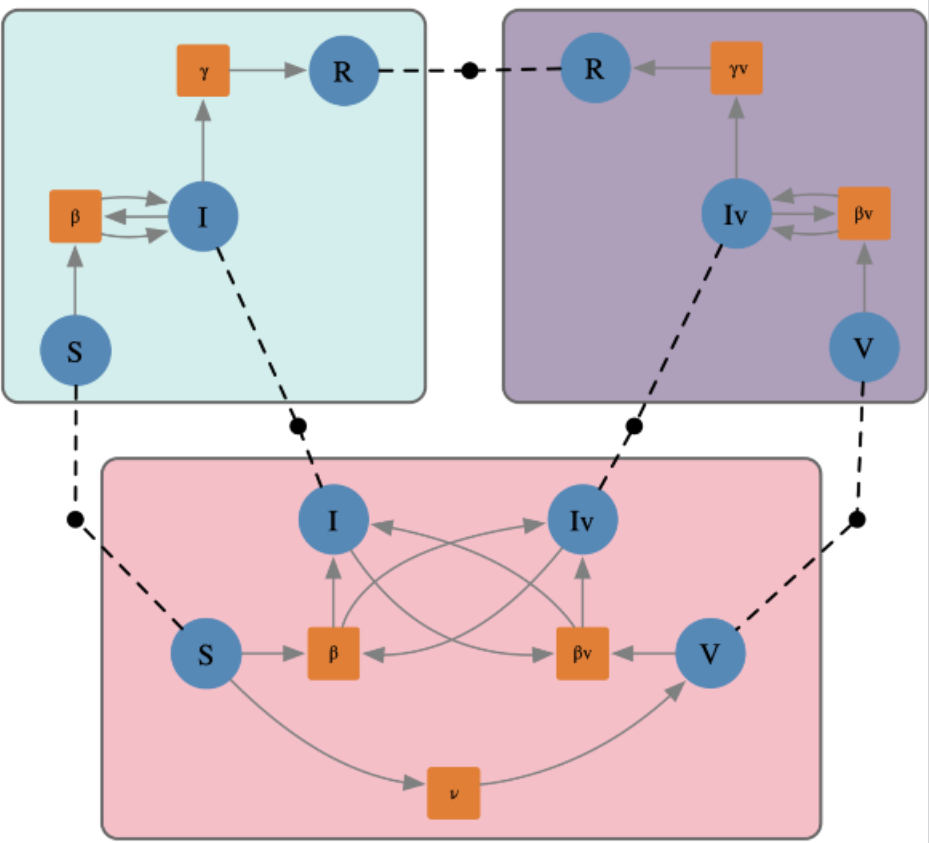
\includegraphics[width=\textwidth]{sub_models}
     \caption{Relating multiple knowledge discovery processes together}
     \label{fig:a}
 \end{subfigure}
 \hfill
 \begin{subfigure}{0.4\textwidth}
     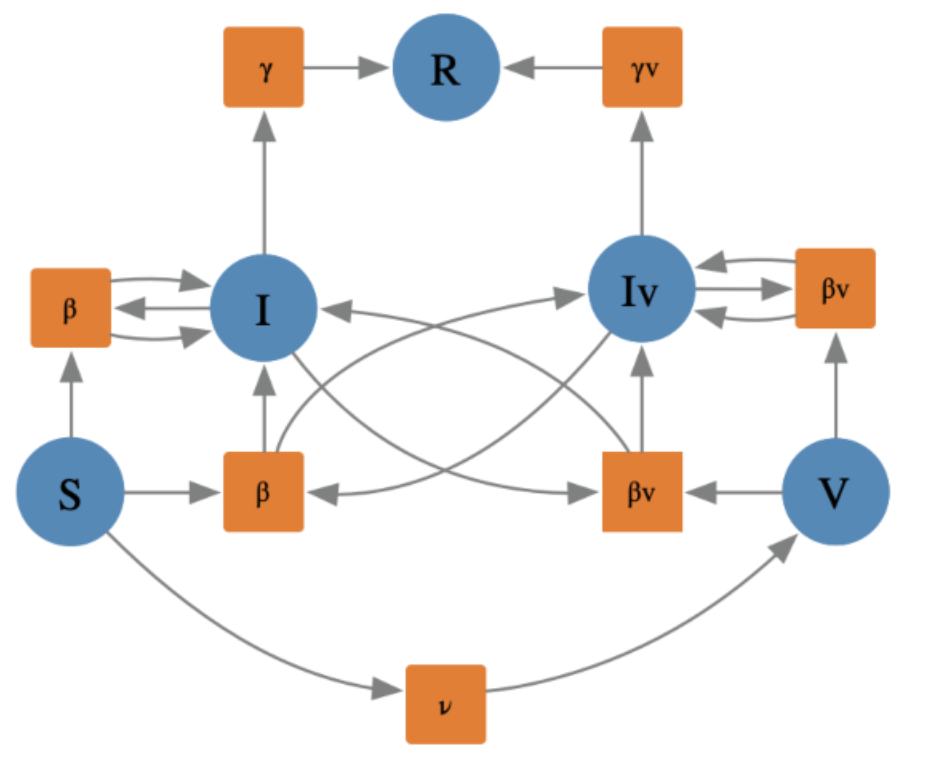
\includegraphics[width=\textwidth]{composed_model}
     \caption{Composing a final process that incorporates information from previous knowledge discovery processes}
     \label{fig:b}
 \end{subfigure}
 \label{Label}

\end{figure}

\textbf{Intellectual Merit:} This project aims to advance approaches in knowledge discovery by leveraging category theory formalizations to observe novel relationships present between knowledge products. 
The use of category theory to harmonize heterogeneous datasets across knowledge discovery processes could offer a new perspective in how traditional discovery could be applied on top of data scaffolded in a category theory framing.
Additionally, by taking advantage of this framing, prior knowledge discovery pipelines could be reused and combined into novel pipelines to address changing needs in engineering or other applied contexts. 

\textbf{Broader Impacts:} By viewing knowledge discovery processes as compositional objects, this could revolutionize how complex systems are analyzed across various disciplines.
Furthermore, as the limits of applied category theoretic machinery is explored in the course of this work, new frontiers in applied category theory could be explored.
This could inform the foundational mathematics undergirding any applications while also leading to the creation of computational software based on these insights.
Finally, this framing could improve the construction of knowledge discovery processes from the beginning by allowing one to easily reason about how a given process in development could be composed in the future or with other pipelines while in development.

\textbf{References:} [1] \textit{Compositionality}, 2024. [2] \textit{ACT4ED}, MIT 1.S980 [3] \textit{Algebraic Databases}, Shultz, et. al., 2016. [4] \textit{Category theory in machine learning}, Gavranović, 2021. [5] \textit{Measuring the impact of knowledge loss: a longitudinal study} Massingham [6] \textit{Emergency Preparedness for Vulnerable Populations}, Nick


\end{document}
